\documentclass[11pt]{article}
\usepackage[margin=0.9in]{geometry}
\usepackage{amsmath,amssymb,amsthm,mathtools}
\usepackage{graphicx}
\usepackage[colorlinks=true,linkcolor=blue,citecolor=blue,urlcolor=blue]{hyperref}
\usepackage{microtype}

\newtheorem{theorem}{Theorem}
\newtheorem{lemma}{Lemma}
\newtheorem{corollary}{Corollary}
\newcommand{\ellone}{\ell_1}
\newcommand{\elltwo}{\ell_2}

\title{An operator range in $\ell_1$ that is not\
an injective operator range}
\author{Candidate full-counterexample packet}
\date{11 August 2026}

\begin{document}
\maketitle

\noindent\textbf{Status.}
Candidate full counterexample; likely valid; human review recommended.

\section{Source question}

Rosenthal and Troitsky use the following finite-power definition.  A linear
subspace $Y$ of a Banach space $X$ is an \emph{operator range} if
$Y=T(M)$ for a bounded operator $T:M\to X$, where $M$ is a closed subspace
of $X^n$ for some finite $n$.  It is an \emph{injective operator range} if
such a presentation can be chosen with $T$ one-to-one.  Remark~4.4 of
\cite{RT} asks whether every operator range in a Banach space is injective in
this sense.  The exact source passage (PDF page~13) is reproduced below.

\begin{center}
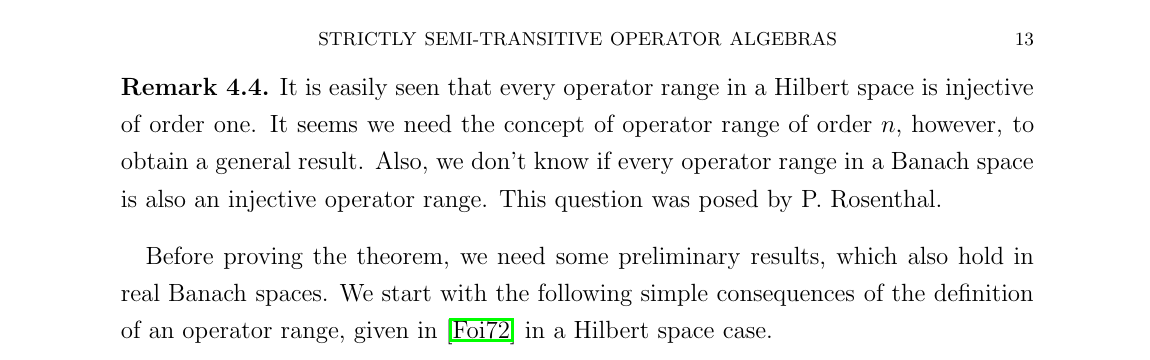
\includegraphics[width=0.98\textwidth]{figures/open_question_crop.png}
\end{center}

The answer is no, already for an order-one range in $X=\ell_1$.

\section{Proof intuition}

The construction separates the Banach space used to \emph{generate} a range
from the ambient geometry allowed in an injective presentation.  The space
$\ell_2$ is a quotient of $\ell_1$, and it admits a bounded one-to-one
diagonal map $J$ into $\ell_1$.  Composing a quotient
$Q:\ell_1\twoheadrightarrow\ell_2$ with $J$ therefore makes $J(\ell_2)$ an
operator range in $\ell_1$.

If the same set were the range of an injective operator from a closed subspace
$N$ of a finite power of $\ell_1$, the two parametrizations would give a
linear bijection $N\to\ell_2$.  Although the inverse of $J$ is not continuous
on its range with the ambient $\ell_1$ norm, the equality of the two
parametrizations makes this bijection closed.  The closed graph and open
mapping theorems then force $N\cong\ell_2$.  This is impossible: every closed
subspace of a finite power of $\ell_1$ has the Schur property, whereas
$\ell_2$ does not.

\section{A general quotient--embedding obstruction}

\begin{lemma}\label{lem:criterion}
Let $X$ and $Z$ be Banach spaces.  Suppose that for some finite $r$ there are
a closed subspace $M\subseteq X^r$, a bounded surjection $Q:M\to Z$, and a
bounded injection $J:Z\to X$.  Put $Y=J(Z)$.  Then $Y$ is an operator range
in $X$.

If $Y$ is an injective operator range, then $Z$ is isomorphic to a closed
subspace of $X^s$ for some finite $s$.
\end{lemma}

\begin{proof}
The bounded map $JQ:M\to X$ has range $J(Z)=Y$, proving the first assertion.

For the second, suppose that $N\subseteq X^s$ is closed and
$S:N\to X$ is bounded and one-to-one with $S(N)=Y$.  Define
\[
                       U=J^{-1}S:N\longrightarrow Z.
\]
This is a well-defined linear bijection.  It has closed graph.  Indeed, if
$u_k\to u$ in $N$ and $Uu_k\to z$ in $Z$, then continuity of $S$ and $J$
gives
\[
        Su=\lim_k Su_k=\lim_k J(Uu_k)=Jz.
\]
Since $J$ is injective, $Uu=z$.  The closed graph theorem makes $U$ bounded,
and the open mapping theorem makes $U^{-1}$ bounded.  Hence $N\cong Z$.
\end{proof}

\section{The $\ell_1$ counterexample}

We include a construction of the standard quotient needed below.

\begin{lemma}\label{lem:quotient}
There is a bounded linear surjection $Q:\ell_1\to\ell_2$.
\end{lemma}

\begin{proof}
Choose a sequence $(u_k)$ in the unit sphere of $\ell_2$ such that every tail
is dense, and define
\[
            Q(a)=\sum_{k=1}^{\infty}a_k u_k
            \qquad(a\in\ell_1).
\]
Then $\|Q\|\leq1$.  Given $x\in\ell_2$, set $r_0=x$.  Recursively, whenever
$r_{j-1}\ne0$, choose a strictly increasing index $k_j$ so that
\[
 \left\|\frac{r_{j-1}}{\|r_{j-1}\|_2}-u_{k_j}\right\|_2<\frac12,
 \qquad
 r_j=r_{j-1}-\|r_{j-1}\|_2u_{k_j}.
\]
Thus $\|r_j\|_2<2^{-j}\|x\|_2$ and
$\sum_j\|r_{j-1}\|_2\leq2\|x\|_2$.  The vector $a\in\ell_1$ with
$a_{k_j}=\|r_{j-1}\|_2$ and all other coordinates zero therefore satisfies
$Q(a)=x$.
\end{proof}

\begin{theorem}\label{thm:counterexample}
There is a bounded operator $T:\ell_1\to\ell_1$ whose range is not an
injective operator range of any finite order in the sense of \cite{RT}.
Consequently, the question in Remark~4.4 of \cite{RT} has a negative answer.
\end{theorem}

\begin{proof}
Let $Q:\ell_1\twoheadrightarrow\ell_2$ be as in
Lemma~\ref{lem:quotient}, and define the bounded injection
\[
 J:\ell_2\longrightarrow\ell_1,
 \qquad J(x_1,x_2,\ldots)=(2^{-1}x_1,2^{-2}x_2,\ldots).
\]
Boundedness follows from Cauchy--Schwarz:
\[
 \|Jx\|_1\leq
 \left(\sum_{k=1}^{\infty}4^{-k}\right)^{1/2}\|x\|_2.
\]
Put $T=JQ$ and $Y=T(\ell_1)=J(\ell_2)$.  Hence $Y$ is an order-one
operator range in $\ell_1$.

If $Y$ were an injective operator range, Lemma~\ref{lem:criterion} would make
$\ell_2$ isomorphic to a closed subspace $N$ of $(\ell_1)^s$ for some finite
$s$.  Finite products of $\ell_1$ have the Schur property, and that property
passes to closed subspaces and is preserved under Banach-space isomorphisms.
But $\ell_2$ does not have the Schur property: its unit vectors converge
weakly to zero and not in norm.  This contradiction proves the theorem.
\end{proof}

\section{Verification, scope, and literature boundary}

The counterexample is stronger than merely requiring a complicated initial
domain: $Y$ is the range of the endomorphism $T=JQ$ of $\ell_1$, yet it has no
injective presentation from a closed subspace of \emph{any} finite power of
$\ell_1$.  The proof applies over either the real or complex field.

It is important not to replace the source's definition by the more common
one allowing an arbitrary Banach domain.  Under that broader definition one
can always quotient the original domain by the kernel and obtain an injective
presentation.  The finite-power restriction is exactly what the Schur
obstruction defeats.

A bounded novelty search on 11 August 2026 used the exact source sentence,
``injective operator range'' with the source definition, $\ell_1/\ell_2$
combinations, and the earlier operator-range work of Cross, Ostrovskii, and
Shevchik~\cite{COS}.  It found literature on arbitrary-domain operator ranges
and injective endomorphism ranges, but no exact finite-power-domain
counterexample matching Theorem~\ref{thm:counterexample}.  Because terminology
varies across this literature and the 1995 paper is extensive, novelty
confidence is moderate, not definitive.

\paragraph{Human-review recommendation.}
Check the definition in Remark~4.4 against the quantification over finite
orders.  Then audit the closed-graph step in Lemma~\ref{lem:criterion}; it is
the only point at which the unbounded inverse of $J$ might superficially appear
problematic, and the displayed sequential argument resolves it.

\begin{thebibliography}{9}
\bibitem{RT}
H.~P. Rosenthal and V.~G. Troitsky,
\emph{Strictly semi-transitive operator algebras},
J. Operator Theory \textbf{53} (2005), 315--329;
arXiv:math/0309014.

\bibitem{COS}
R.~W. Cross, M.~I. Ostrovskii, and V.~V. Shevchik,
\emph{Operator ranges in Banach spaces, I},
Math. Nachr. \textbf{173} (1995), 91--114.
\end{thebibliography}

\end{document}
